\documentclass{fkssolpub}

\usepackage[czech]{babel}
\usepackage{fontspec}
\usepackage{fkssugar}
\usepackage{amsmath}
\usepackage{graphicx}

\author{Ondřej Sedláček}
\school{Gymnázium Oty Pavla} 
\series{1}
\problem{A} 

\begin{document}

\begin{figure}
	\begin{center}
		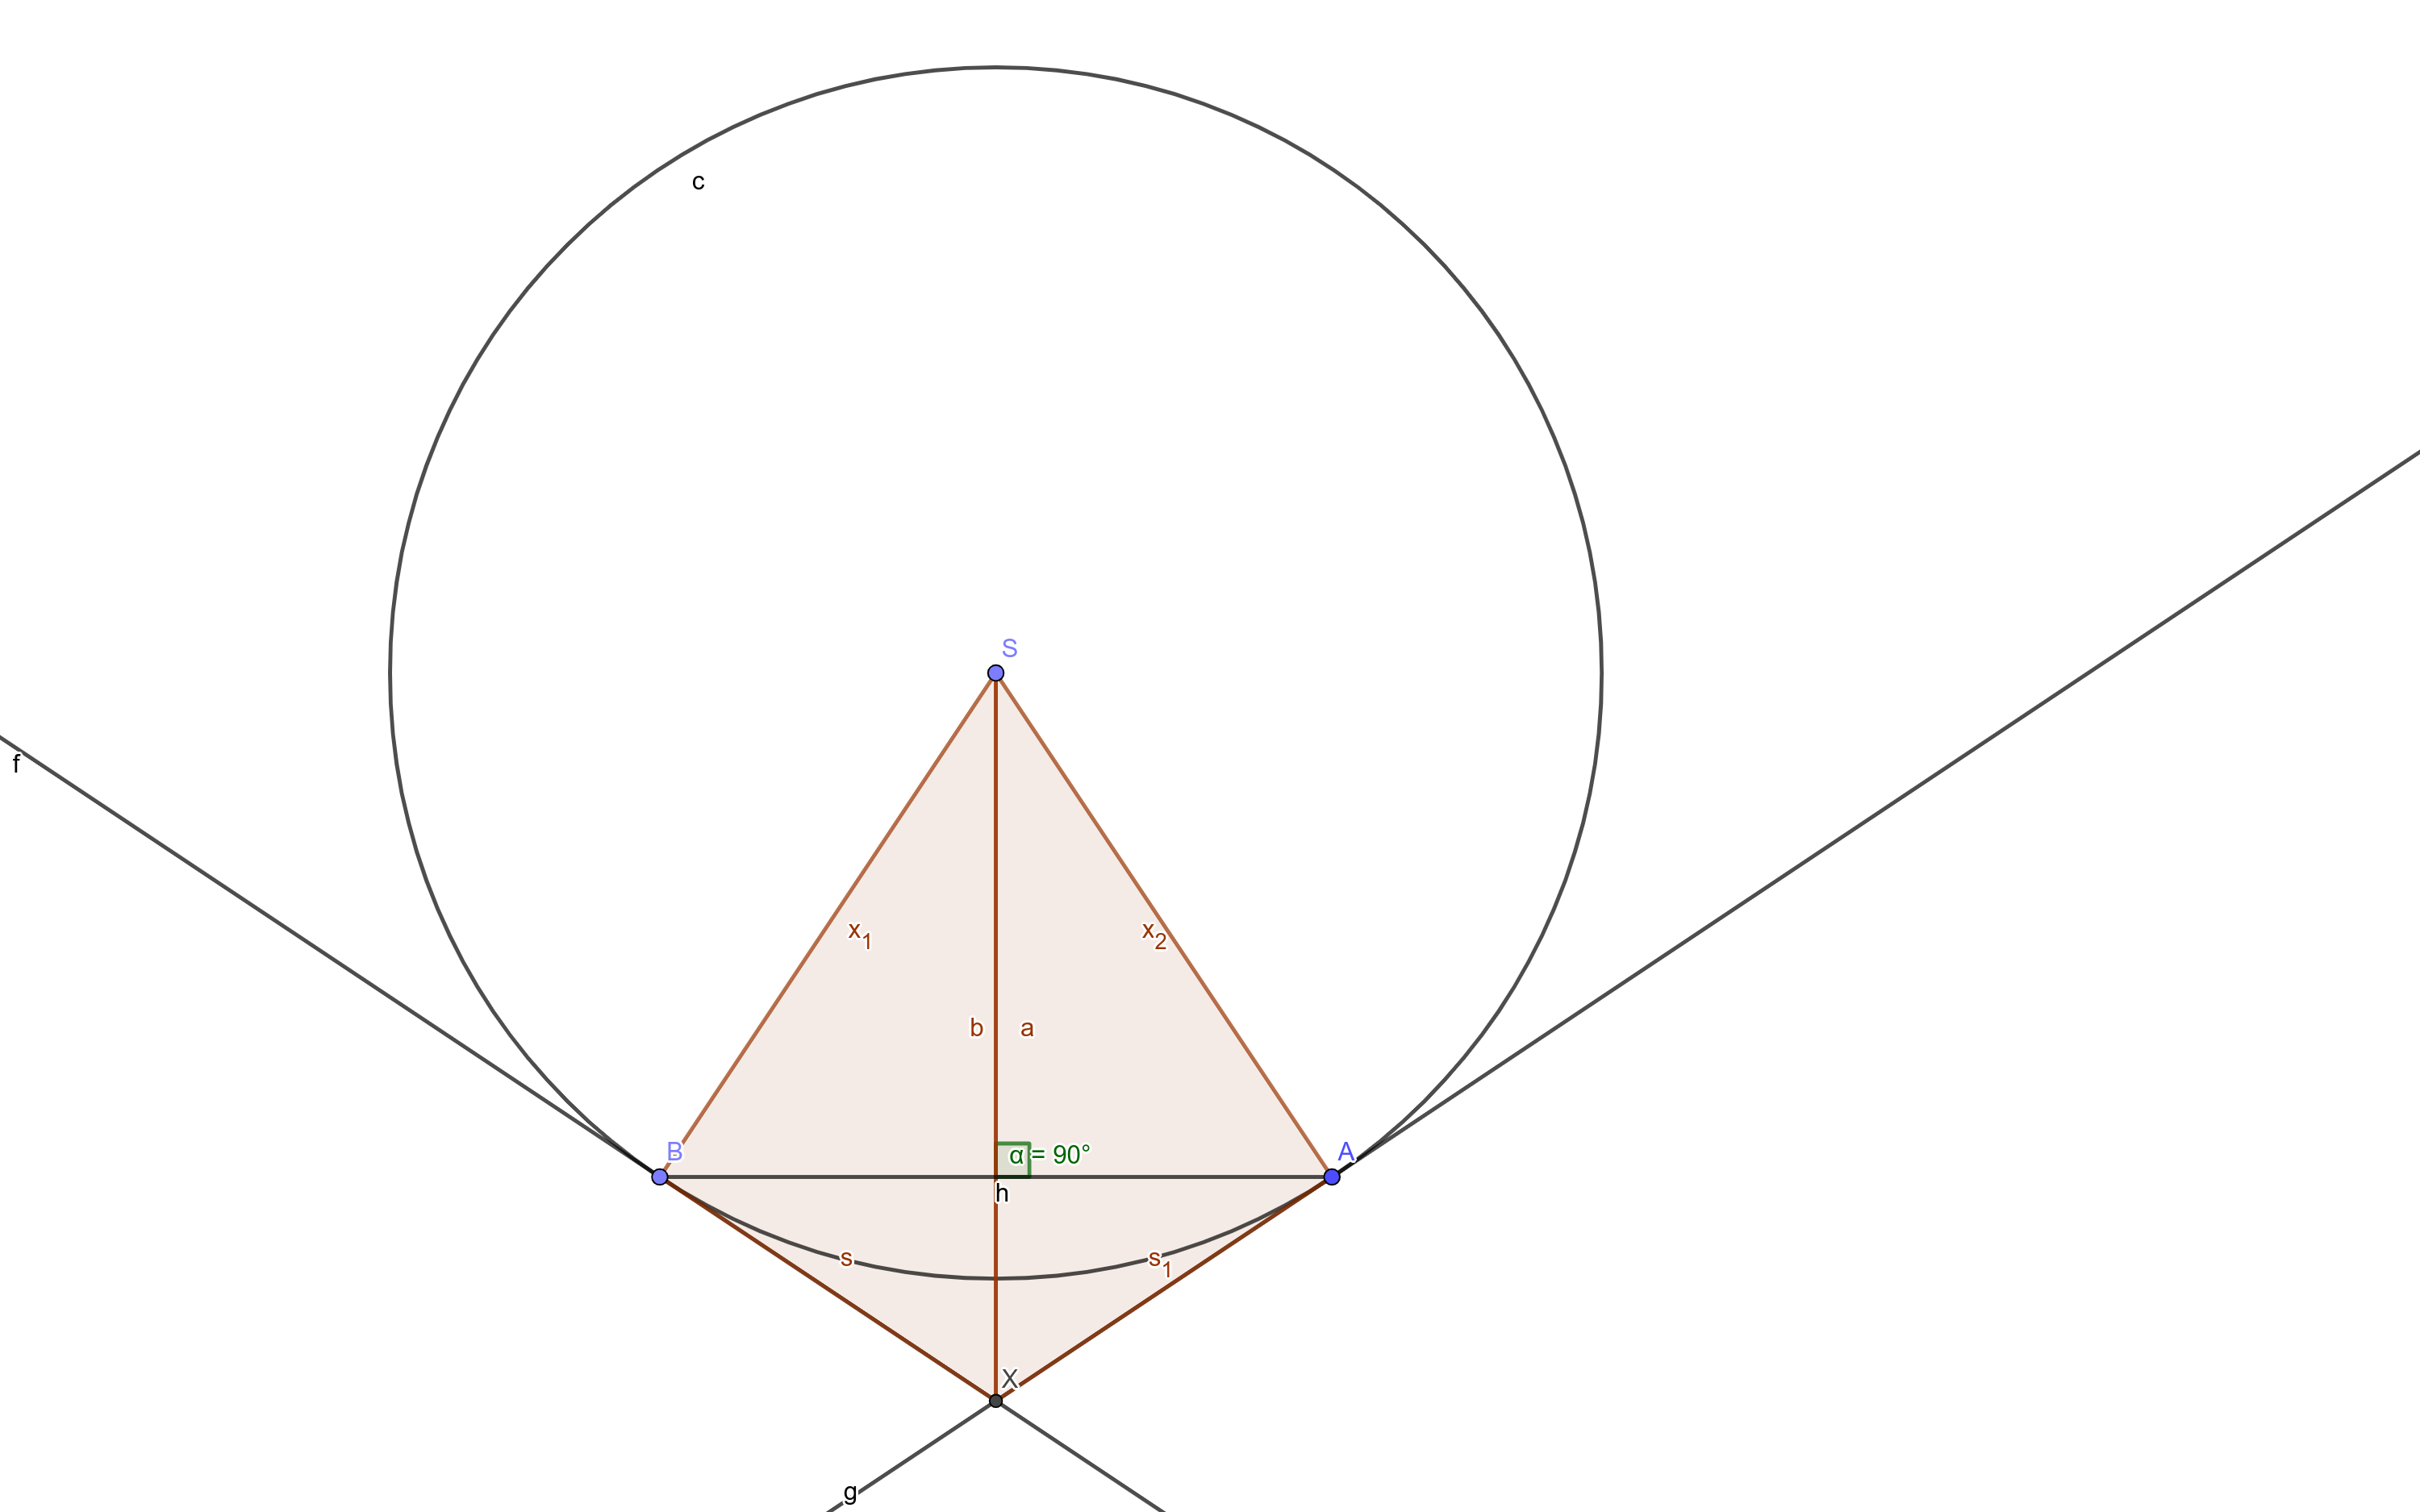
\includegraphics[width=0.95\textwidth]{A-fig}
	\end{center}
	\caption{Konstrukce úlohy}
	\label{fig:1}
\end{figure}

Víme, že trojúhelníky $ABS$ a $BAX$ jsou rovnoramenné, tím pádem jsou trojúhelníky $SXA$ a $XSB$ shodné a jsou v osové souměrnosti. Tím pádem velikost spojnice $AB$ je rovna dvojnásobku výšky těchto trojúhelníků s patou na $XS$. Na vyjádření té výšky použijeme vzorec, který získáme dosazením Euklidových vět o odvěsně do Euklidovy věty o výšce:

\[
	a^2 = c \cdot c_a \ztoho c_a = \frac{a^2}{c}
\]
\[
	b^2 = c \cdot c_b \ztoho c_b = \frac{b^2}{c}
\]
\[
	v^2 = c_a \cdot c_b
\]
\[
	v = \frac{a b}{c}
\]

Tento vzorec následně uplatníme:

\[
	\frac{|AB|}{2} = \frac{r \cdot |AX|}{\sqrt{r^2 + |AX|^2}}
\]
\[
	|AB|^2 \cdot (r^2 + |AX|^2) = 4 r^2 \cdot |AX|^2
\]
\[
	|AB|^2 \cdot r^2 = |AX|^2 (4 r^2 - |AB|^2)
\]
\[
	|AX| = \frac{|AB| \cdot r}{\sqrt{4r^2 - |AB|^2}}
\]

Tím jsme určili vzdálenost $|AX|$.

\end{document}
